% Created 2022-05-20 Fri 17:57
% Intended LaTeX compiler: pdflatex
\documentclass[11pt]{article}
\usepackage{amsmath}
\usepackage[utf8]{inputenc}
\usepackage[T1]{fontenc}
\usepackage{graphicx}
\usepackage{longtable}
\usepackage{wrapfig}
\usepackage{rotating}
\usepackage[normalem]{ulem}
\usepackage{amsmath}
\usepackage{amssymb}
\usepackage{capt-of}
\usepackage{hyperref}
\usepackage{listings}
\usepackage[margin=2cm]{geometry}
\usepackage{enumitem}
\usepackage{tikz}
\usepackage{fancyvrb}
\date{}
\title{Beating Amdahl's Law with Parallel Self-adjusting Data Structures}
\hypersetup{
 pdfauthor={},
 pdftitle={Beating Amdahl's Law with Parallel Self-adjusting Data Structures},
 pdfkeywords={},
 pdfsubject={},
 pdfcreator={Emacs 27.1 (Org mode 9.5.2)}, 
 pdflang={English}}
\begin{document}

\maketitle
\setitemize{noitemsep,topsep=0pt,parsep=0pt,partopsep=0pt}
\fvset{baselinestretch=.5,samepage=true,xleftmargin=1cm,fontsize=\small}

\section{Abstract}
\label{sec:org672edee}
One major obstacle faced by network engineers is how to harness the massive computing power, which
increasingly comes in the form of parallel processing cores, given that Amdahl's law predicts
diminishing returns for massive-scale parallelization.  Using three simple illustrative models, we
show that the combination of \emph{locality-boosting load-balancing} and \emph{parallel self-adjusting data
structures} allows to achieve superlinear scaling for some typical massively parallel networking
workloads. We demonstrate quadratic scale-up in certain cases and, strikingly, we show that
parallelization yields linear scaling even if we keep the total available computing power constant.

\section{Introduction}
\label{sec:orge0719da}
\begin{itemize}
\item simply put, Amdahl's law states that throwing additional processors to a fixed-size parallel
computation will yield diminishing returns
\item Amdahl's law is usually stated in terms of speedup, but it can be interpreted in the usual
goodput vs. CPU-cores coordinate system as well.
\end{itemize}

\begin{center}
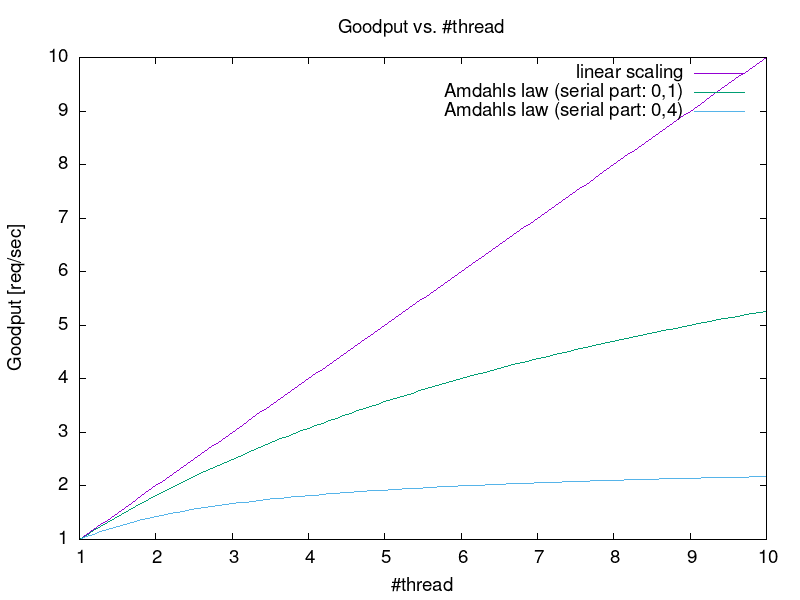
\includegraphics[width=9cm]{usl.png}
\end{center}

\section{Motivation}
\label{sec:orgeb571da}

\begin{itemize}
\item the pattern "distribute requests to a set of concurrent worker threads" is fairly familiar in
networking
\begin{itemize}
\item endhost network stacks: NIC hashes packet headers and RSS distributes packets based on the hash
across a set of CPUs
\item HTTP load-balancers with "sticky sessions": split requests based on the source IP and allocate
each to a backend server, same user will always end up at the same backend
\item sharded key-value stores (like REDIS): client splits queries based on the key-hash, each shard
handles only a subset of the hash-space
\item anything else?
\end{itemize}
\item this pattern has proved remarkably useful: since networking workloads are typically massively
parallel, with minimal need for synchronization across the threads, we usually get linear
speed-up
\item of course, the load-balancer is still serial so Amdahl's law curtails max performance at the
load-balancer's throughput
\item we argue that there is even more to this model than we would have thought, which may even yield
superlinear speedup for careful implementations
\item this is made possible by the unique combination of two important components, locality boosting
load-balancing and self-adjusting worker threads, that may further improve efficiency even
without us being aware
\end{itemize}

\subsection{Locality boosting load-balancing}
\label{sec:org8d49eee}
\begin{itemize}
\item the idea in all use-cases above is that requests to the same or "similar" items are processes at
the same worker: 5-tuple hashes in RSS, per-source-IP load-splitting in HTTP load-balancers,
key-hashes in sharded key-value stores, they always keep similar jobs at the same worker (TODO:
make this argument more precise!)
\item this improves temporal and/or spatial locality as experienced by the worker threads
\item round-robin or random load-balancing promote locality in the input to the workers: not "locality
boosting"
\item hash-based load-balancing or range-based splitting: improves locality (TODO: can we reason about
this in simple terms?)
\end{itemize}

\subsection{Self-adjusting data structures}
\label{sec:org6cf39c7}
\begin{itemize}
\item a self-adjusting data structure can rearrange itself as queries are committed to it in order to
improve efficiency on future requests
\item exploit locality of reference in the input
\item red-black trees or AVL trees rearrange with respect to the stored data to keep the search tree
balanced: not self-adjusting
\end{itemize}

\subsection{Idea}
\label{sec:org591e535}
\begin{itemize}
\item a locality boosting load-balancer splits requests so that worker threads experience improved
locality of reference
\item self-adjusting data structures at the workers exploit the improved locality in the input they
process
\item the more threads the greater the locality in the per-thread request sequences, and the more
efficient the self-adjustments
\item the superlinear scaling thanks to self-adjustments initially outweigh the slowdowns predicted by
Amdahl's law
\item eventually of course Amdahl's law kicks in and performance saturates, but up to that point we
expect superlinear scaling
\end{itemize}

\section{Case Studies}
\label{sec:orgfa6e163}

\subsection{Model}
\label{sec:org2122015}
\begin{itemize}
\item a source emits requests (jobs) for \(m\) items (we assume a uniform source below)
\item a job scheduler (essentially a load-balancer) allocates the requests to workers
\item \(k\) parallel worker threads running on \(n\le k\) CPU cores
\item models implemented in Go, evaluated on a 24-core Intel x86 server
\end{itemize}

\begin{verbatim}
                                     +--------+
                              +----->|Thread 1|
                              |      +--------+
                              |
                              |      +--------+
+------+    +-------------+   +----->|Thread 2
|Source|----|Load-balancer|---+      +--------+
+------+    +-------------+   |          .
                              |          .
                              |          .
                              |      +--------+
                              +----->|Thread k|
                                     +--------+
\end{verbatim}

\subsection{Caching}
\label{sec:org431b585}
\begin{itemize}
\item simplest self-adjusting data-structure: LRU cache
\item we get caches by default in all current CPUs, but many networking applications explicitly contain
a fast-path/cache component: key-value stores [ebpf/NSDI], FIB caching [linux], flow-caches as a
fast-path in OvS, etc.
\item strikingly, caches alone, paired with a locality boosting load-balancer (like RSS), can already
provide superlinear scaling as we show below
\end{itemize}
\subsubsection{Analysis}
\label{sec:org8279ab1}
\begin{itemize}
\item lookup time: \(l = \delta + (1-\delta)\rho\), where \(\delta\) is the cache hit rate and \(\rho\) is
the cost of a cache miss; we assume \(\delta=.025\) and \(\rho=100\)
\item if all requests are processed on a single thread, that thread will experience a cache hit rate of
\(\delta\) on \(m\) items
\item if the request set is randomly split into \(k\) partitions, then the working set at each thread
reduces to \(\frac{m}{k}\) and so we expect the cache hit rate to increase to \(k\delta\) at each of
the threads
\item lookup time on \(k\) threads: \(l_k = k\delta + (1-k\delta)\rho = \rho - k\delta(\rho-1)\)
\item throughput on \(k\) threads: \(t_k = \frac1{l_k} = \frac1{\rho - k\delta(\rho-1)}\)
\item throughput on \(n\) cores with \(k\ge n\) threads: \(t_k(n) = \frac{n}{\rho - k\delta(\rho-1)}\)
\item for \(n=k\) this yields superlinear \(O(\frac{k}{b - k})\) scaling
\end{itemize}

\subsubsection{Multicore scaling}
\label{sec:org9a71096}
\begin{itemize}
\item \(n=k\): superlinear scaling confirmed
\end{itemize}

\begin{center}
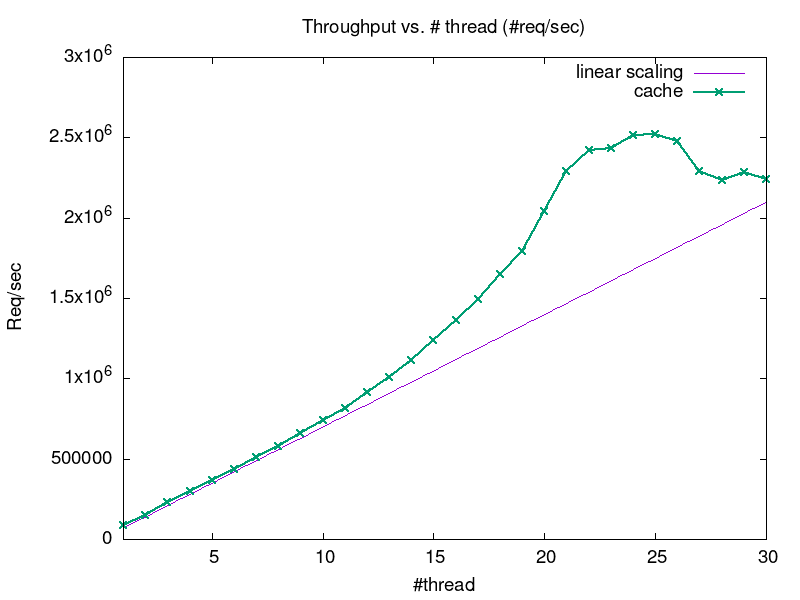
\includegraphics[width=9cm]{cache-no-cpu-bound.png}
\end{center}

\subsubsection{Scaling on a single core}
\label{sec:orgb79cc1d}
\begin{itemize}
\item \(n=1\): we see a linear yield for running \(k\) parallel threads even if we restrict the system to a
single CPU core
\end{itemize}

\begin{center}
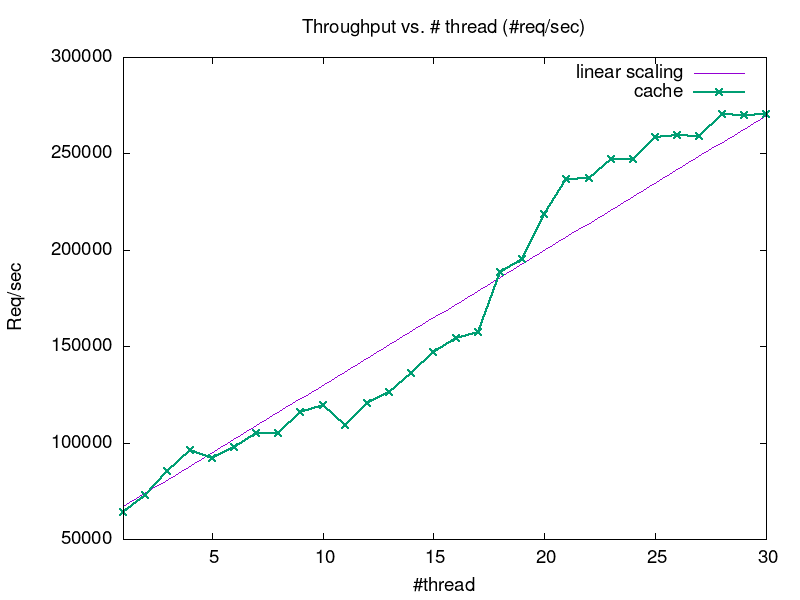
\includegraphics[width=9cm]{cache-cpu-bound-150.png}
\end{center}

\subsection{Move-to-front lists}
\label{sec:org378fced}
\begin{itemize}
\item classical applications: information retrieval
\item networking: packet classification, ternary flow tables, intrusion detection
\end{itemize}

\subsubsection{Analysis}
\label{sec:orgb4914dd}
\begin{itemize}
\item average lookup time on one thread is \(\frac1{2}m\), where the working-set size equals \(m\)
\item randomly splitting items to \(k\) partitions also partition the working sets, yielding \(l_k =
  \frac{m}{2k}\) lookup time
\item throughput on \(k\) threads: \(t_k = \frac1{l_k} = \frac{2 k}{m}\)
\item throughput on \(n\) cores with \(k\ge n\) threads: \(t_k(n) = \frac{2k n}{m}\)
\item for \(n=k\) this yields \(O(k^2)\) scaling
\end{itemize}

\subsubsection{Multicore scaling}
\label{sec:orga8c51b3}
\begin{itemize}
\item \(n=k\)
\end{itemize}
\begin{center}
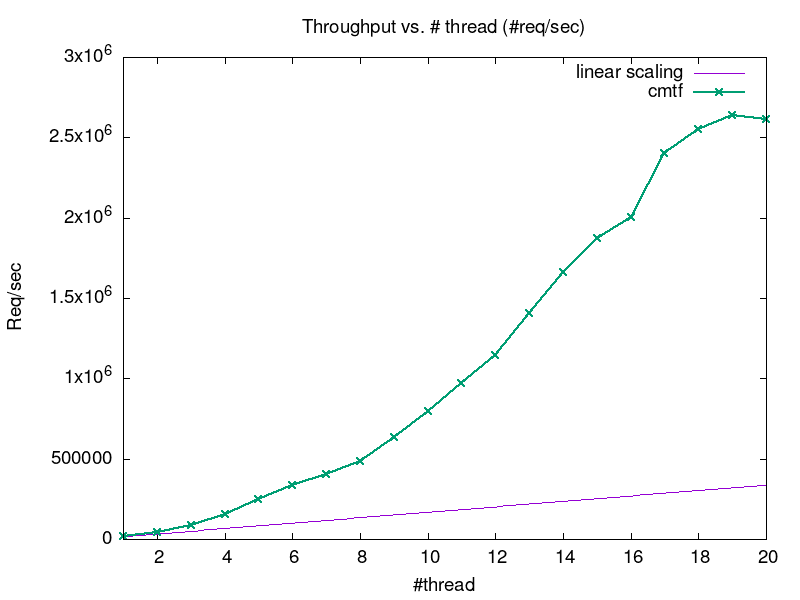
\includegraphics[width=9cm]{cmtf-no-cpu-bound.png}
\end{center}

\subsubsection{Scaling on a single core}
\label{sec:orgd1770c1}
\begin{itemize}
\item \(n=1\)
\end{itemize}
\begin{center}
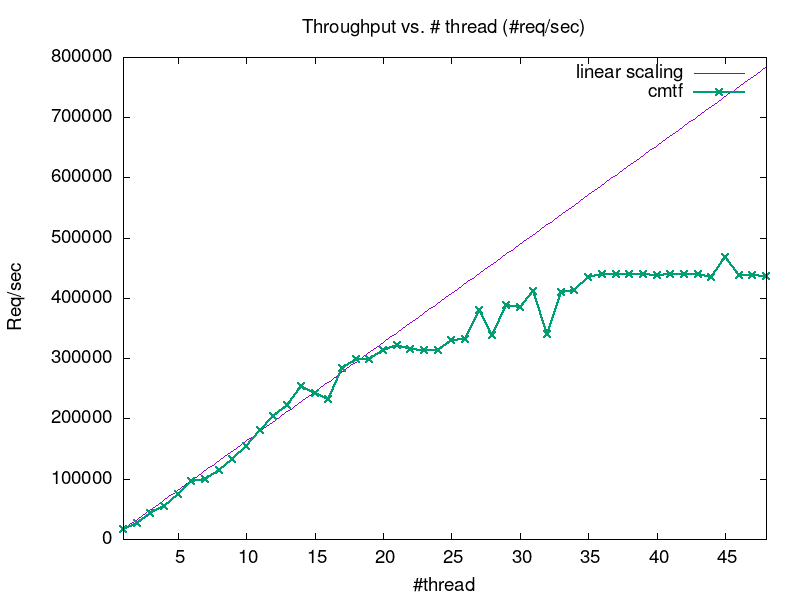
\includegraphics[width=9cm]{cmtf-cpu-bound-150.png}
\end{center}

\subsection{Splay tree}
\label{sec:org3e4aad2}
\begin{itemize}
\item networking applications: maybe FIB lookups?
\end{itemize}

\subsubsection{Multicore scaling}
\label{sec:orgd1eb1a1}
\begin{itemize}
\item \(n=k\)
\end{itemize}

\begin{center}
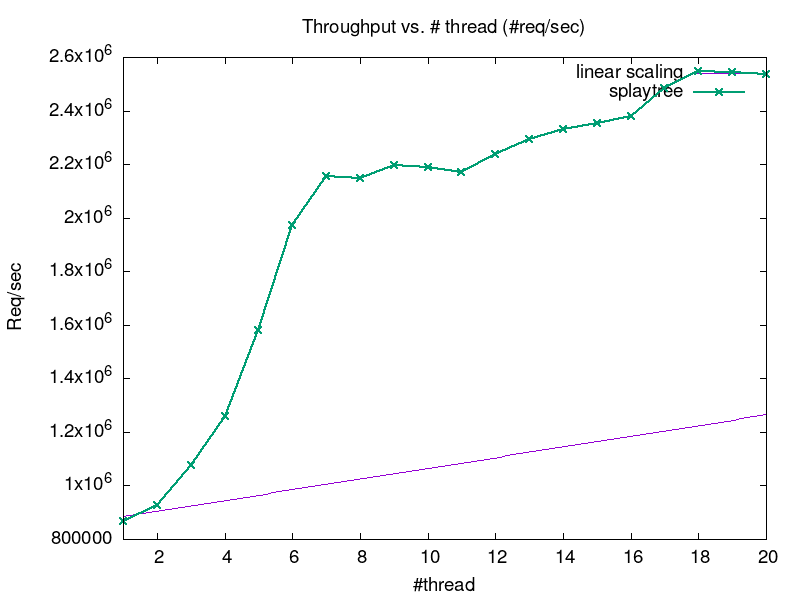
\includegraphics[width=9cm]{splay-no-cpu-bound.png}
\end{center}

\subsubsection{Scaling on a single core}
\label{sec:orgf3e8461}
\begin{itemize}
\item \(n=1\)
\end{itemize}

\begin{center}
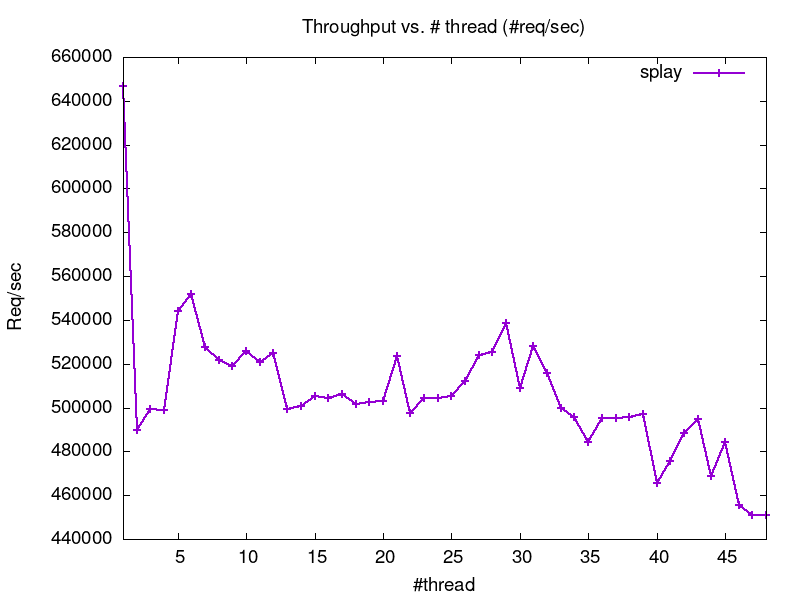
\includegraphics[width=9cm]{splay-cpu-bound-150.png}
\end{center}
\end{document}
